%% Template article for Elsevier's document class `elsarticle`
%% with numbered style bibliographic references
\documentclass[preprint,12pt, a4paper]{elsarticle}

\usepackage{amssymb}
\usepackage{amsmath}
\usepackage{hyperref}
\usepackage{booktabs}
\usepackage{graphicx}
\usepackage{xcolor}
\usepackage{orcidlink}
\usepackage{longtable}
\usepackage{float}
\usepackage{tabularx}
\setlength{\parindent}{0pt}

\journal{SoftwareX}

\begin{document}
\renewcommand{\labelenumii}{\arabic{enumi}.\arabic{enumii}}

\begin{frontmatter}

\title{A Modular NLU-Solr Architecture with Dynamic GIS Visual Synchronization for Conversational Spatial Search}

\author[1]{F{\'e}lix de Miguel \orcidlink{0009-0000-9607-110X}\corref{cor1}}
\ead{fdemiguel@ubu.es}

\author[1]{Daniel Urda \orcidlink{0000-0003-2662-798X}}
\ead{durda@ubu.es}

\author[1]{Nu{\~n}o Basurto \orcidlink{0000-0001-7289-4689}}
\ead{nbasurto@ubu.es}

\cortext[cor1]{Corresponding author at: Grupo de Inteligencia Computacional Aplicada (GICAP), Departamento de Digitalizaci{\'o}n, Escuela Polit{\'e}cnica Superior, Universidad de Burgos, Av. Cantabria s/n, 09006 Burgos, Spain.}

\address[1]{Grupo de Inteligencia Computacional Aplicada (GICAP), Departamento de Digitalizaci{\'o}n, Escuela Polit{\'e}cnica Superior, Universidad de Burgos, Av. Cantabria s/n, 09006 Burgos, Spain}

\begin{abstract}
Navigating complex geospatial data spaces through conventional search portals presents substantial friction for domain users, requiring rigid query syntax or exposing interfaces to Large Language Model (LLM) database schema hallucinations. Moreover, in strategic domains such as Critical Raw Materials (CRMs), relying on external commercial cloud APIs introduces severe data sovereignty and confidentiality risks. In this paper, we present a domain-agnostic, modular open-source software architecture connecting a dual-variant Natural Language Understanding (NLU) pipeline with Apache Solr spatial indexing and dynamic Geographic Information System (GIS) map visual synchronization. The architecture establishes a synchronized map-and-chat interface, enabling users to translate free-form natural language queries directly into deterministic, visually synchronized spatial filtering. To eliminate schema hallucinations between pipeline nodes, the system couples Few-Shot intent parsing with strict OpenAPI JSON Schema enforcement evaluated under greedy decoding. Extracted search parameters are dynamically transformed into structured Boolean filter queries, simultaneously rendering active visual filter badges and triggering animated glowing pulse markers across the cartographic interface. The software natively supports both zero-setup standalone mock execution and on-premises local execution of open-weight foundation models (Llama 3.2 3B, Qwen 2.5 7B, Phi-3 Mini 4K) on private GPU infrastructure, guaranteeing 100\% European data sovereignty. To demonstrate its practical applicability, the architecture is instantiated and evaluated within \textbf{CRMsDataSpace}, a European research initiative for Critical Raw Materials. Empirical evaluation across 40 critical stress tests and 100 domain queries on an NVIDIA A100 testbed demonstrates high extraction accuracy (up to 93.1\% macro F1-score across local GPU models and 96.6\% overall accuracy), establishing a secure, reproducible foundation for sovereign conversational GIS exploration.
\end{abstract}

\begin{keyword}
Geographic Information Systems (GIS) \sep Software Architecture \sep Natural Language Understanding (NLU) \sep Large Language Models (LLMs) \sep Spatial Data Search \sep Data Sovereignty \sep Common European Data Spaces
\end{keyword}

\end{frontmatter}

\section*{Required Metadata}
\label{sec:Metadata}

\begin{longtable}{|l|p{6.5cm}|p{6.5cm}|}
\hline
\textbf{Nr.} & \textbf{Code metadata description} & \textbf{Metadata} \\
\hline
C1 & Current code version & v1.0.0 \\
\hline
C2 & Permanent link to code/repository used for this code version & \url{https://github.com/felixdmv/CRMsDataSpace-SoftwareX} \\
\hline
C3 & Legal Code License & MIT License \\
\hline
C4 & Code versioning system used & git \\
\hline
C5 & Software code languages, tools, and services used & Python 3.9+, HTML5, JavaScript (Leaflet.js), TailwindCSS, Apache Solr (SolrCloud / Standalone), PyTorch (CUDA 12), Hugging Face Transformers, Google Gemini API \\
\hline
C6 & Compilation requirements, operating environments \& dependencies & Standard Python 3.9+ library (Standalone Mock Mode); Optional for production retrieval: Apache Solr 9.x+ (SolrCloud cluster or Standalone); Optional for GPU acceleration: NVIDIA GPU with CUDA 12 (A100, RTX 3080/4080+), PyTorch, Transformers; Optional cloud: Google Generative AI SDK, OpenAI API client \\
\hline
C7 & Link to developer documentation/manual & \url{https://github.com/felixdmv/CRMsDataSpace-SoftwareX/blob/main/README.md} \\
\hline
C8 & Support email for questions & \href{mailto:fdemiguel@ubu.es}{fdemiguel@ubu.es} \\
\hline
\caption{Code metadata (mandatory)}
\label{tab:metadata}
\end{longtable}

%% Modular Sections
\section{Motivation and significance}
\label{sec:MotivationAndSignificance}

Modern Geographic Information Systems (GIS) and domain-specific data spaces manage vast volumes of multi-attribute spatial, environmental, and observational records~\cite{curry2022data}. Interacting with these platforms typically requires users to navigate complex relational schemas, master rigid query syntax (such as SQL or Lucene), or execute dozens of manual filter selections across multi-level nested web forms~\cite{huang2022natural, dou2024survey}. This introduces substantial cognitive friction, limits exploratory spatial inquiry, and prevents non-technical domain stakeholders from effectively discovering relevant geographic assets.

Recent breakthroughs in Large Language Models (LLMs) and conversational artificial intelligence have created promising opportunities for natural language querying in geospatial domains (GeoAI)~\cite{janowicz2020geoai, mai2023opportunities, li2023geollm}. However, deploying unconstrained LLMs over spatial databases introduces three severe impediments: (i)~\textbf{Database Schema Hallucination}, where models invent non-existent attribute names or relational keys~\cite{dou2024survey, willard2023outlines}; (ii)~\textbf{Non-Deterministic Output Structures}, producing unparseable payloads that break downstream database APIs~\cite{willard2023outlines, pydantic2023}; and (iii)~\textbf{Absence of Geospatial Visual Feedback}, isolating users in text streams without cartographic synchronization~\cite{scheider2021question, huang2022natural}.

To bridge this gap, this paper presents a generic, modular, open-source software architecture connecting a dual-variant Natural Language Understanding (NLU) pipeline, Apache Solr structured spatial indexing, and dynamic Geographic Information System (GIS) map visual synchronization. The architecture is domain-agnostic: by establishing clean functional boundaries between intent parsing, terminology normalization, search index querying, and cartographic rendering, the pipeline can be instantiated across diverse spatial disciplines by modifying only the domain thesaurus and the OpenAPI schema specification.

\begin{table}[h!]
    \centering
    \small
    \setlength{\tabcolsep}{5pt}
    \caption{Comparative analysis of the proposed NLU-Solr-GIS architecture against existing spatial search and conversational AI approaches.}
    \label{tab:tool_comparison}
    \begin{tabularx}{\linewidth}{>{\raggedright\arraybackslash\bfseries}p{3.4cm}>{\raggedright\arraybackslash}X>{\raggedright\arraybackslash}X>{\raggedright\arraybackslash}X}
        \toprule
        \textbf{Dimension} & \textbf{Traditional GIS} & \textbf{Raw LLMs / Text-to-SQL} & \textbf{Proposed Architecture} \\
        \midrule
        Query Modality & Rigid forms / Dropdowns & Free-form natural text & Conversational spatial NLU \\
        Hal\-lu\-ci\-na\-tion Risk & None (Static controls) & High (Invented attributes) & \textbf{Zero (OpenAPI Schema)} \\
        Output Determinism & High & Low (Stochastic output) & \textbf{Guaranteed (Validated JSON)} \\
        GIS Map Feedback & Manual navigation & None (Text-only stream) & \textbf{Real-Time Pulse \& Badges} \\
        Domain Lexicon & Exact string matching & Latent / Unpredictable & \textbf{Pluggable Thesaurus} \\
        Data Sovereignty & Local database & Low (External cloud APIs) & \textbf{100\% On-Premises GPU} \\
        Repro\-duci\-bil\-i\-ty & Live database required & External API key required & \textbf{Standalone Mock Mode} \\
        \bottomrule
    \end{tabularx}
\end{table}

\subsection{Case Study and Validation Testbed: The CRMsDataSpace European Project}
\label{subsec:CaseStudyContext}

To demonstrate the practical applicability of the proposed architecture within a demanding, real-world deployment, the software is instantiated and validated within \textbf{CRMsDataSpace}, a European research project funded by the Research Fund for Coal and Steel (Grant Agreement No.~101216677). 

The objective of the CRMsDataSpace initiative is to establish a Common European Data Space on Critical Raw Materials (CRMs) for the European Green Deal~\cite{european2024crma, blengini2020eu}. The project characterises closed extractive waste facilities, tailings ponds, and spoil heaps across Europe as secondary mineral sources to support EU supply resilience~\cite{vidal2017environmental, lottermoser2010mine}. Within this ecosystem, our software architecture serves as the conversational front-end of the Minimum Viable Data Space (MVDS), allowing mining engineers, geologists, and policymakers to query multi-criteria spatial and mineralogical records in natural language with synchronized cartographic feedback. The CRMs domain acts as an exemplary case study highlighting the versatility and robustness of the generic software pattern.

\section{Software description}
\label{sec:SoftwareDescription}

The proposed software architecture is engineered as a decoupled, modular system designed to bridge conversational natural language processing, spatial search engine indexing, and interactive web mapping. The design prioritizes strict separation of concerns, defensive programming against LLM hallucinations, and immediate cartographic visual feedback.

\subsection{Software Architecture Overview}
\label{subsec:SoftwareArchitecture}

The architecture is structured around four decoupled execution stages, as illustrated in the workflow diagram in Figure~\ref{fig:arch}.

\begin{figure}[h!]
\centering
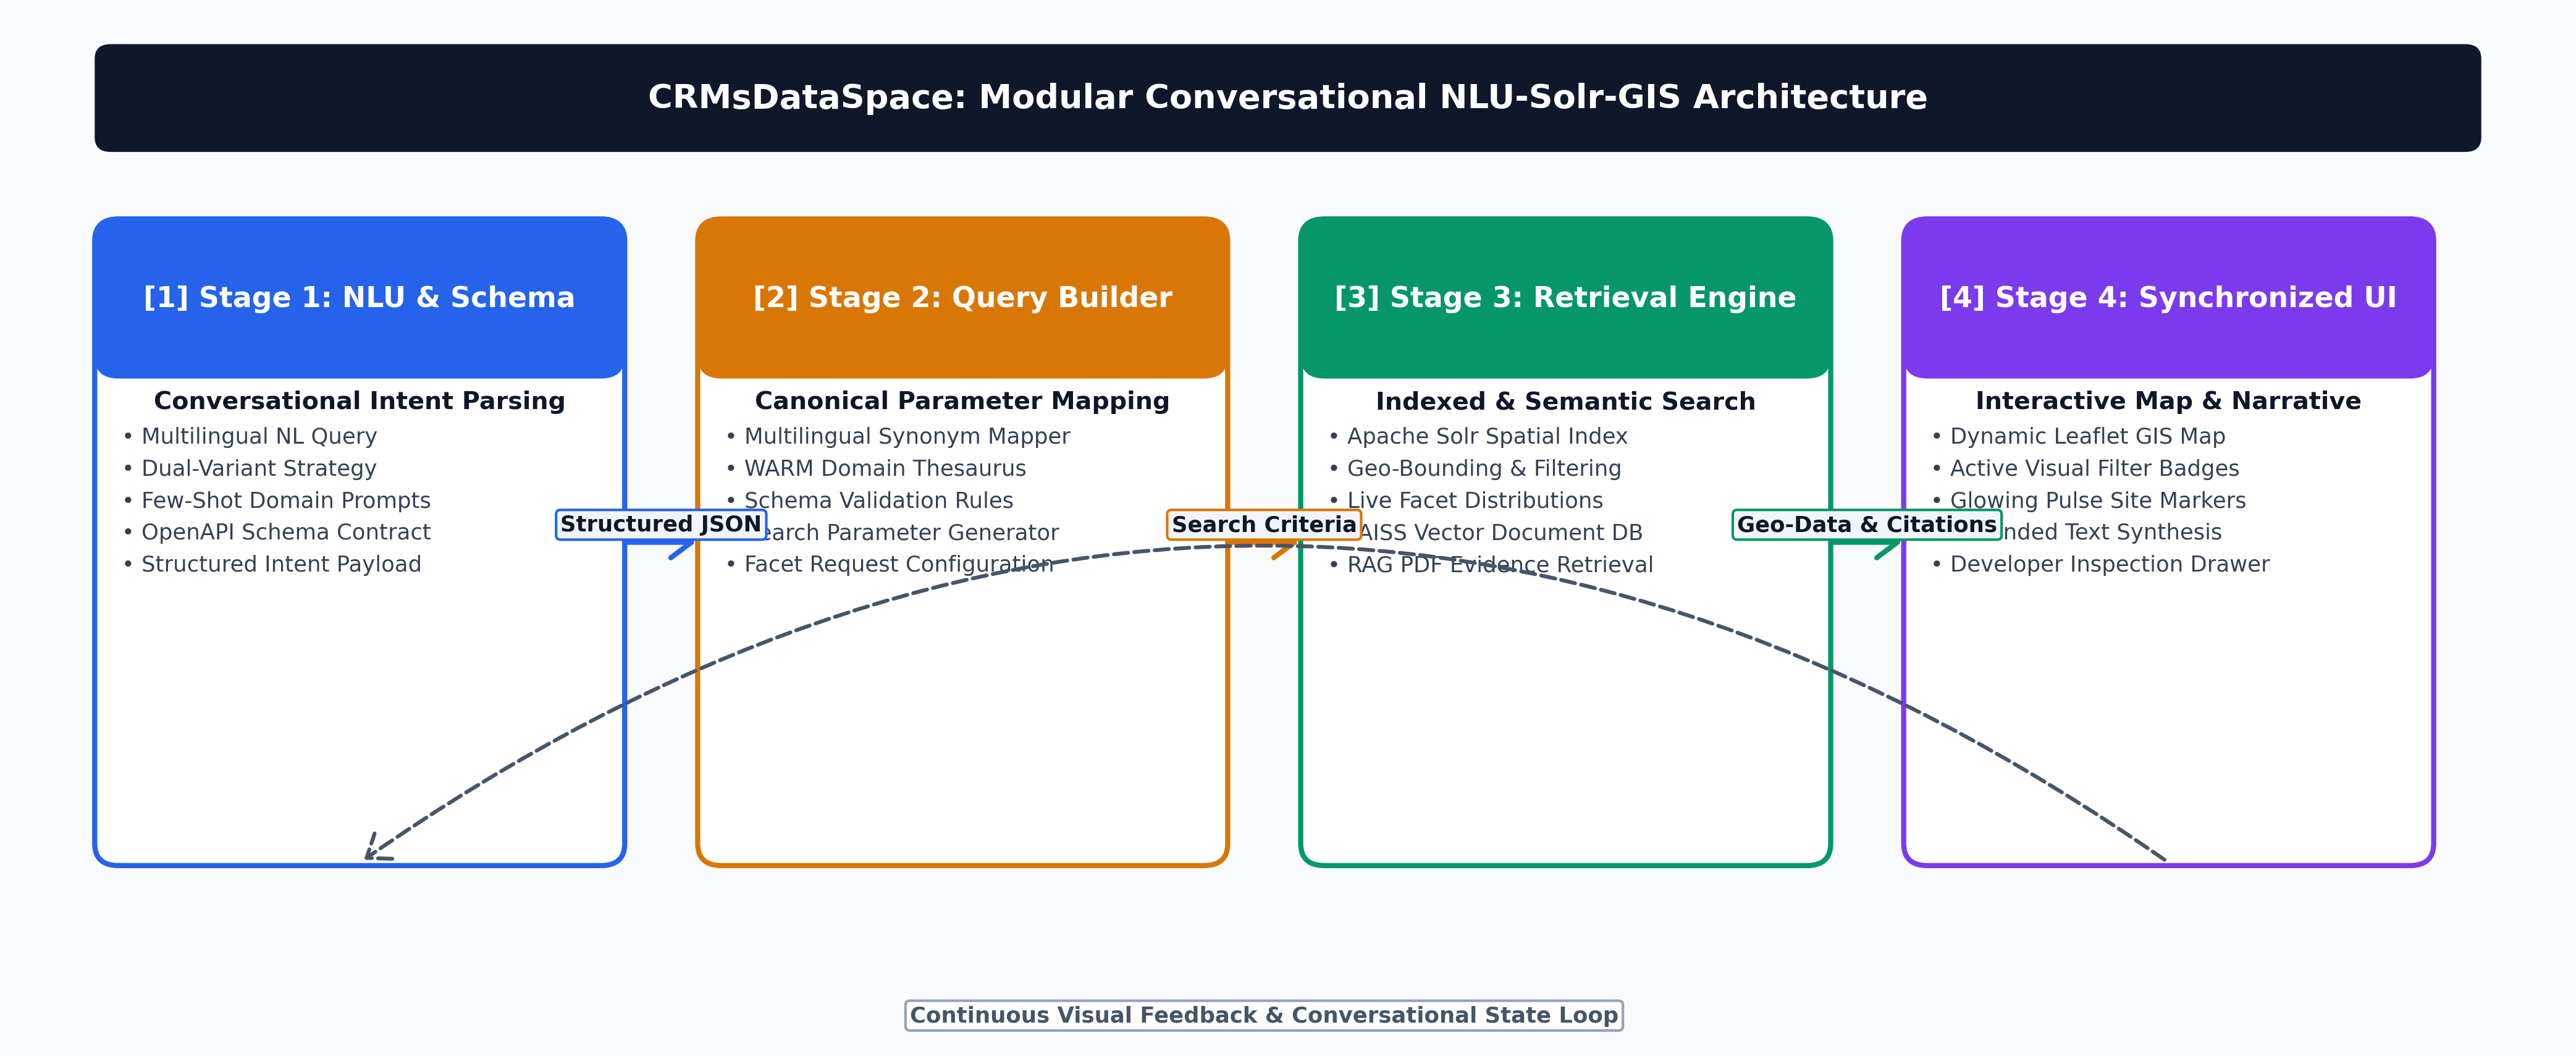
\includegraphics[width=0.98\textwidth]{architecture_diagram.png}
\caption{Overall decoupled software pipeline architecture combining conversational NLU intent parsing, query generation, spatial search engine retrieval, and dynamic GIS web map synchronization.}
\label{fig:arch}
\end{figure}

The functional workflow operates through four decoupled layers:

\begin{enumerate}
    \item \textbf{Stage 1: Conversational NLU \& Schema Enforcement}: The user submits a free-text spatial query $Q$ through the web interface. Rather than permitting unconstrained text generation, the query is processed by a dual-variant NLU parser that combines Few-Shot contextual exemplars with a strict OpenAPI JSON Schema evaluated under greedy decoding ($T = 0.0$)~\cite{willard2023outlines, gemini2024}. This contract guarantees that the extracted payload strictly adheres to pre-defined intent types and entity slots, completely eliminating database schema hallucinations (Figure~\ref{fig:comp1}).
    
    \begin{figure}[h!]
    \centering
    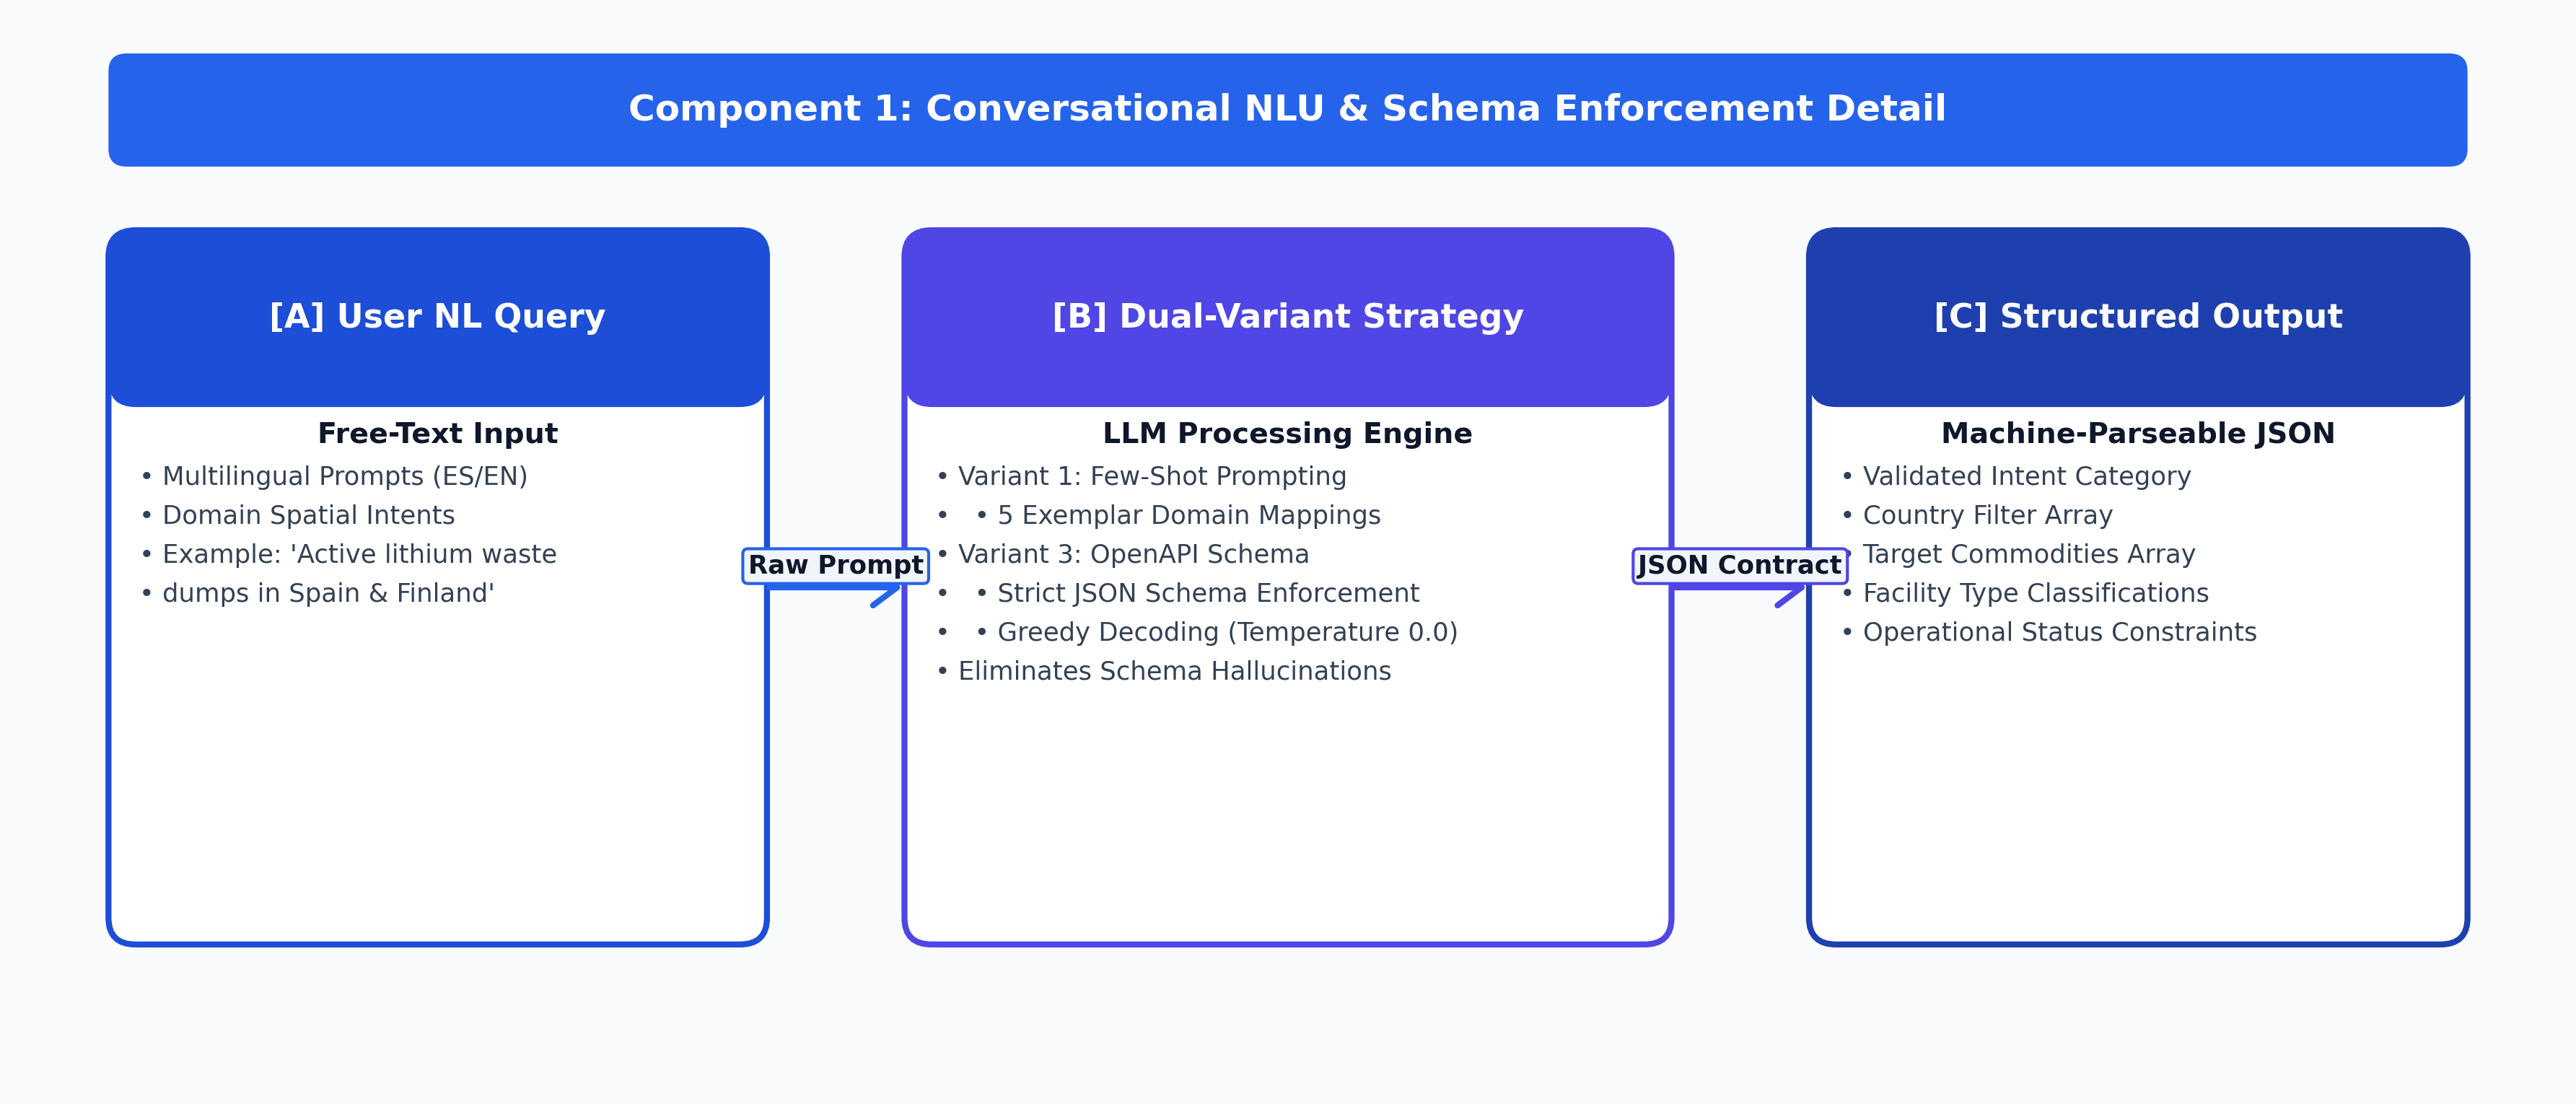
\includegraphics[width=0.90\textwidth]{component1_nlu_schema.png}
    \caption{Workflow of Stage 1: Conversational NLU Intent Parsing with dual-variant Few-Shot prompting and OpenAPI JSON Schema enforcement.}
    \label{fig:comp1}
    \end{figure}

    \item \textbf{Stage 2: Pluggable Domain Normalization \& Search Query Generation}: Extracted entity values frequently contain informal expressions, regional language synonyms, or chemical element symbols. Component~2 routes these values through a pluggable domain thesaurus that normalizes terms into canonical vocabularies aligned with standard reporting taxonomies~\cite{ballatore2014vocabulary}. A schema validator verifies structural integrity before constructing disjunctive and conjunctive Boolean search filter arrays for Apache Solr (Figure~\ref{fig:comp2}).

    \begin{figure}[h!]
    \centering
    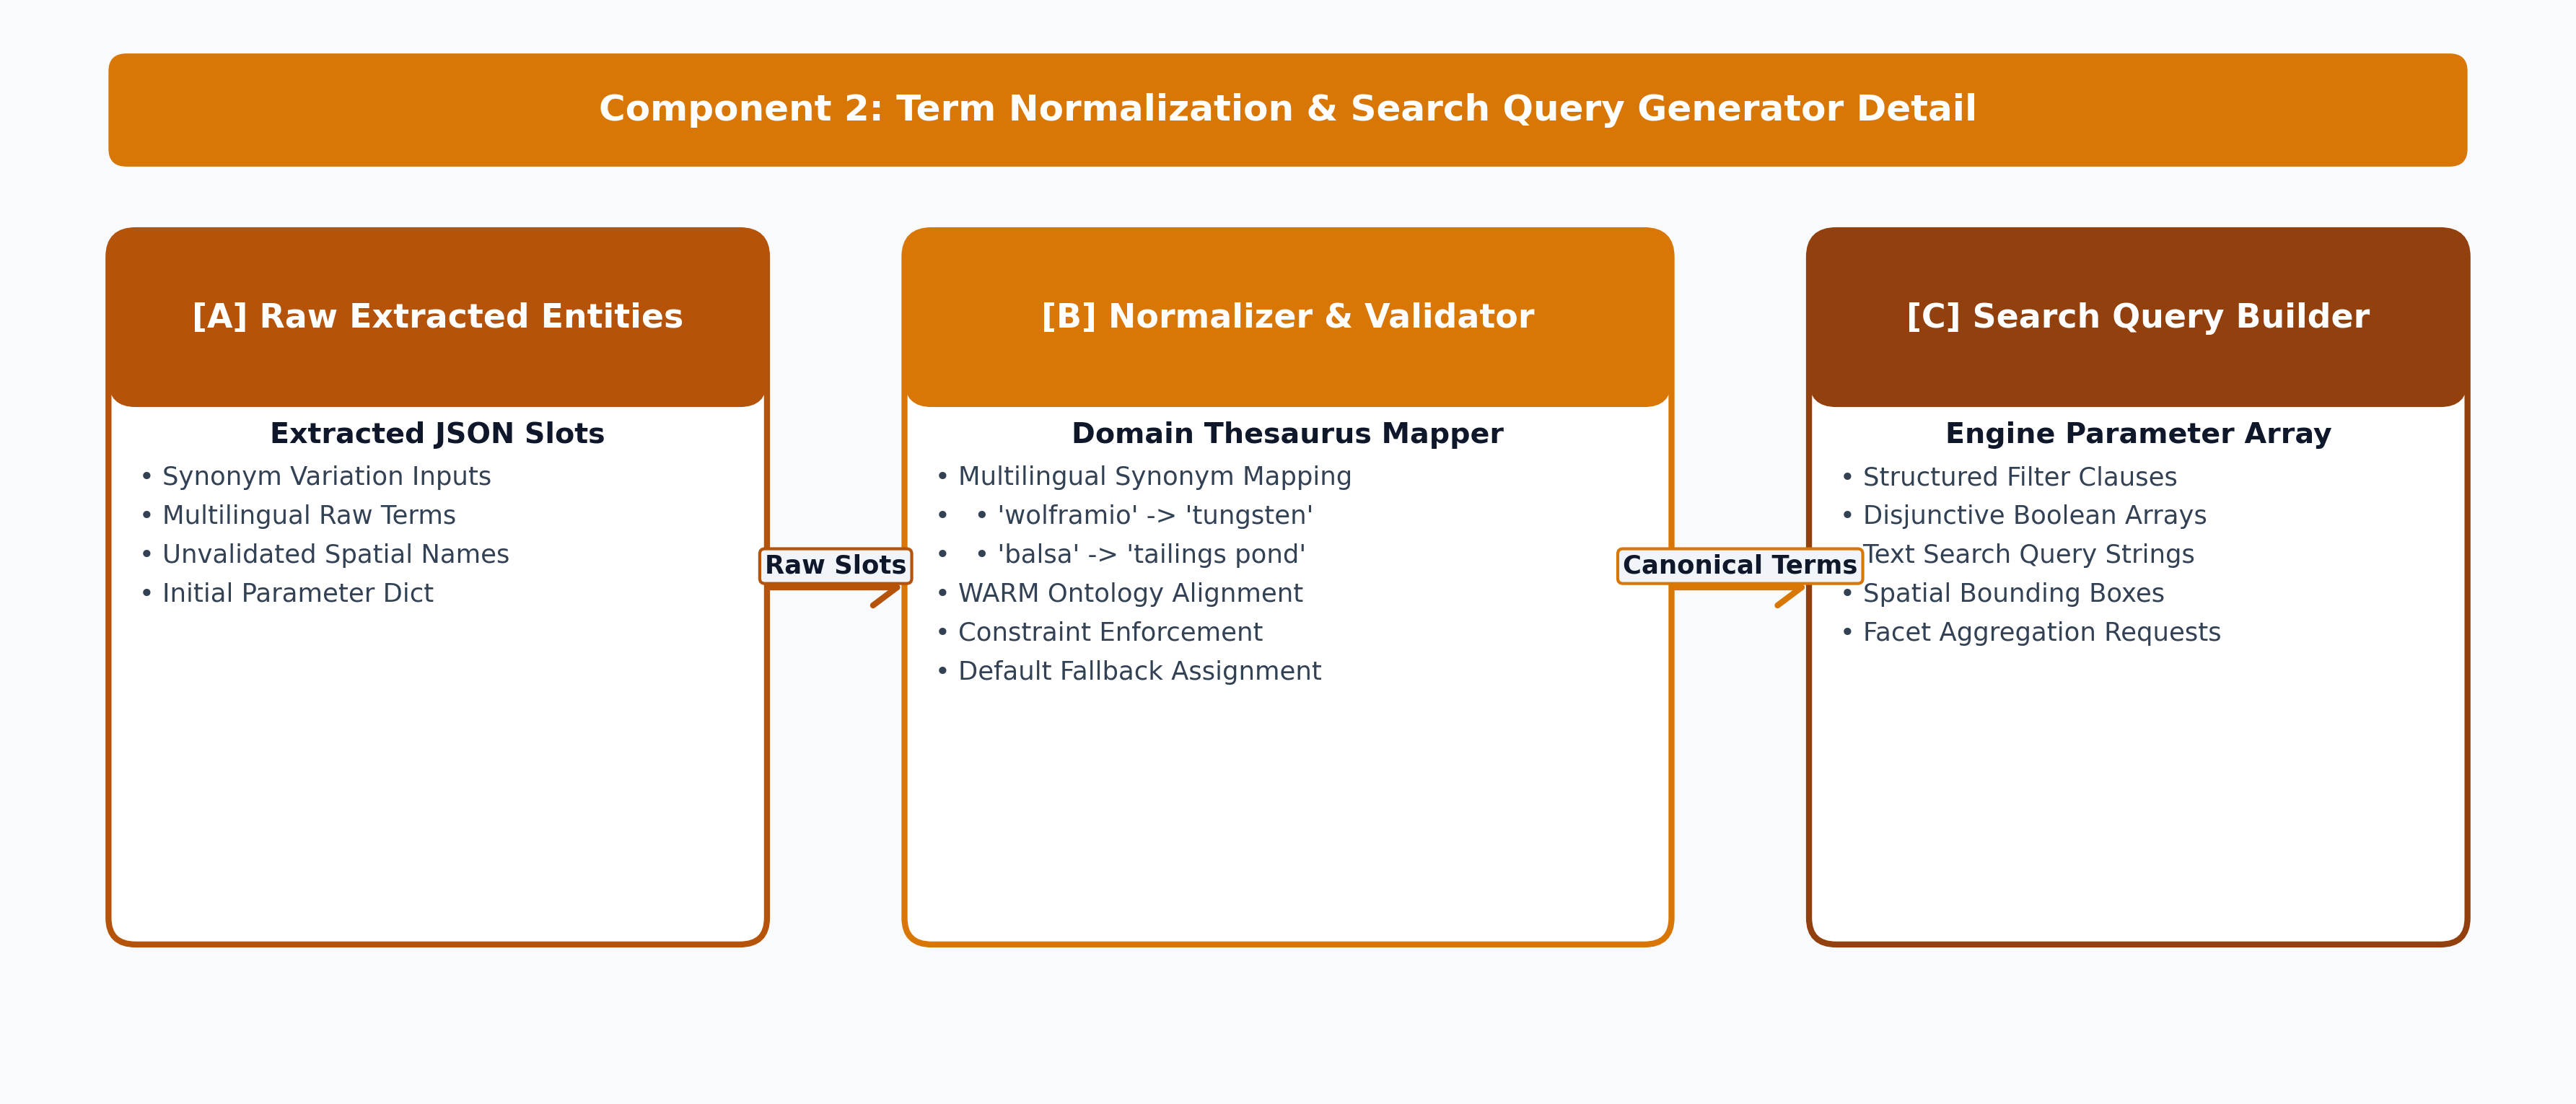
\includegraphics[width=0.90\textwidth]{component2_query_builder.png}
    \caption{Workflow of Stage 2: Multilingual Domain Term Normalization, Validation, and Solr Filter Query Generation.}
    \label{fig:comp2}
    \end{figure}

    \item \textbf{Stage 3: Spatial Search Engine Indexing \& Vector Evidence Retrieval}: The generated filter queries execute against an Apache Solr spatial engine~\cite{solr2020}. In production data spaces such as CRMsDataSpace, the retrieval layer interfaces with a distributed \textbf{SolrCloud} cluster coordinated via Apache ZooKeeper, providing high availability, fault-tolerant horizontal sharding across heterogeneous regional nodes, and automated replication for continent-wide extractive inventories. The software architecture is completely agnostic to the underlying deployment topology: the query generator produces standard Lucene filter parameters (\texttt{q}, \texttt{fq}, and faceting directives over standard HTTP REST endpoints) that interface identically with distributed SolrCloud collections, single-node Solr standalone cores, or the embedded zero-setup standalone mock engine via environment variable configuration (\texttt{SOLR\_URL}). Solr evaluates geospatial constraints using spatial indexing fields (such as \texttt{LatLonPointSpatialField} and bounding box filters) and computes live multi-dimensional facet distributions~\cite{solr2020, manning2008information}. In parallel, when the query requests unstructured technical or regulatory evidence, a dense vector index (FAISS)~\cite{johnson2019billion, lewis2020retrieval} performs similarity retrieval over document chunks, applying an information-density reranker to select top-scoring citation snippets (Figure~\ref{fig:comp3}).

    \begin{figure}[h!]
    \centering
    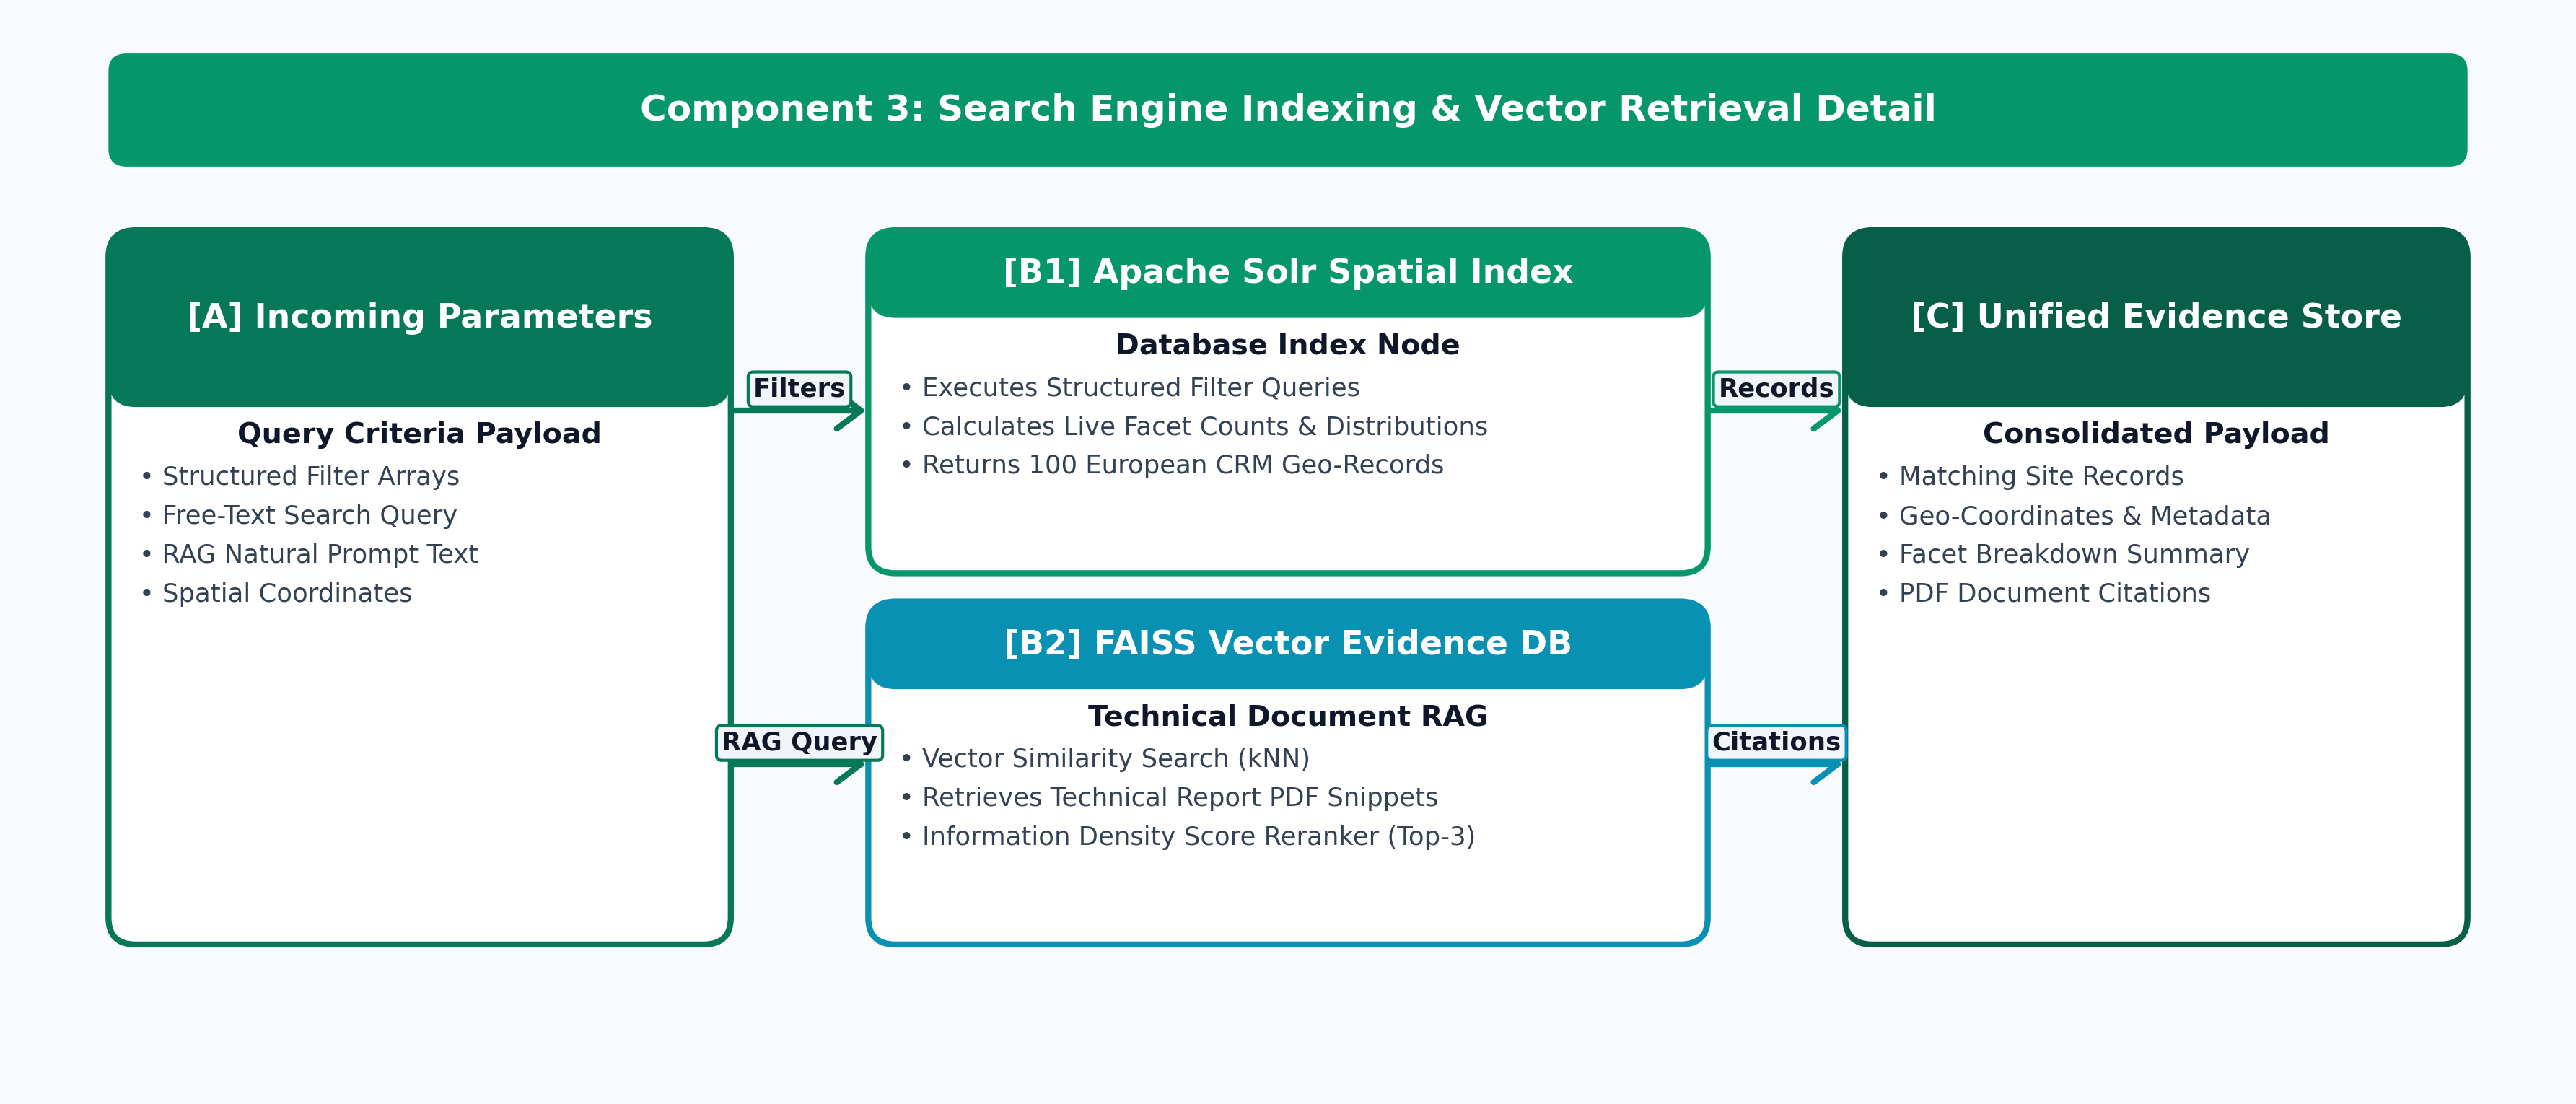
\includegraphics[width=0.90\textwidth]{component3_search_rag.png}
    \caption{Workflow of Stage 3: Dual Spatial Search Engine (Apache Solr) and Technical Document Vector Retrieval (FAISS).}
    \label{fig:comp3}
    \end{figure}

    \item \textbf{Stage 4: Dynamic GIS Map \& Conversational Web Dashboard}: The client web application, built with Leaflet.js~\cite{leaflet2023} and TailwindCSS, receives the consolidated spatial records, facet statistics, and textual evidence. As illustrated in Figure~\ref{fig:comp4}, the interface integrates real-time GPU VRAM telemetry (A), an active visual filter sub-bar (B), dynamic cartography with animated glowing pulse rings (C), a grounded conversational chat assistant with traceable document citations (D), and a slide-out developer inspection drawer (E) providing full transparency into intermediate JSON artifacts and executed Solr parameters.

    \begin{figure*}[t!]
    \centering
    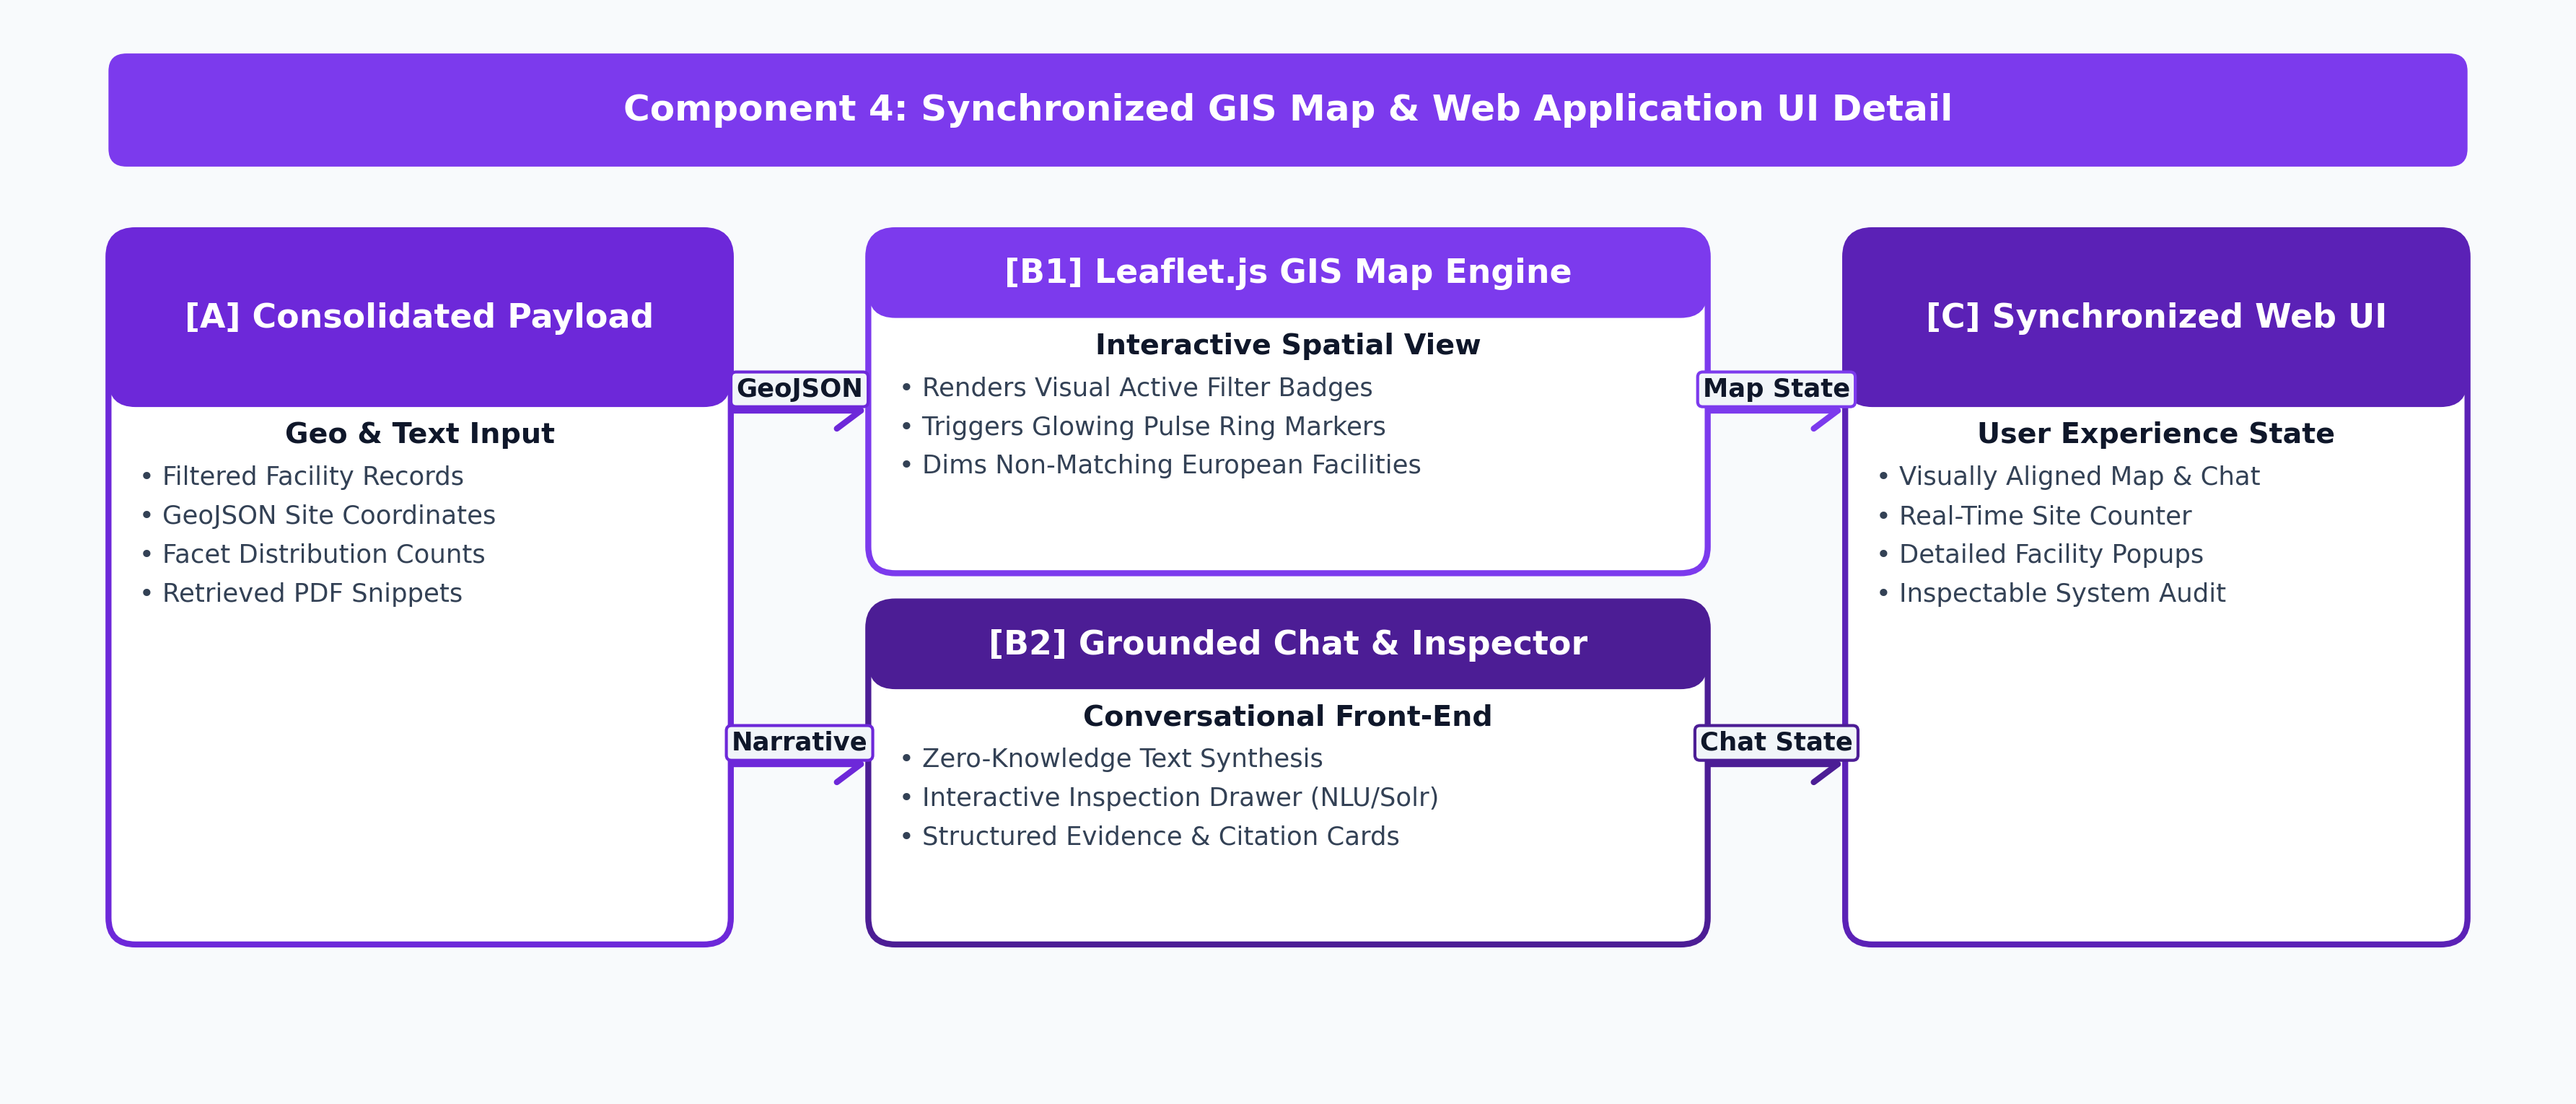
\includegraphics[width=\textwidth]{component4_gis_ui.png}
    \caption{Annotated operational interface of the CRMsDataSpace web demonstrator: (A)~Real-time GPU VRAM telemetry badge monitoring on-premises NVIDIA A100 inference; (B)~Dynamic active visual filter sub-bar translating conversational criteria into filter pills; (C)~Interactive Leaflet.js GIS map with animated glowing pulse markers on matching European CRM waste facilities and popup metadata cards; (D)~Grounded conversational chat synthesizing responses with traceable PDF technical evidence cards; (E)~Slide-out developer inspection drawer for live auditing of intermediate OpenAPI JSON extractions and Solr spatial filter parameters.}
    \label{fig:comp4}
    \end{figure*}
\end{enumerate}

\subsection{Software Functionalities}
\label{subsec:SoftwareFunctionalities}

The software architecture delivers the following general-purpose capabilities:

\begin{itemize}
    \item \textbf{Multi-Criteria Natural Language Filtering}: Users can formulate complex queries combining geographic boundaries, domain commodities/categories, physical facility types, and operational/environmental conditions.
    \item \textbf{Dynamic GIS Visual Synchronization \& Multi-Select Attribute Widget}: Extracted search criteria are converted into interactive visual badges on the map header and automatically populate a floating multi-selection attribute panel. Users can toggle multiple jurisdictions (e.g., cross-border queries spanning Spain and Portugal) or commodities manually with immediate two-way state synchronization. The map viewport dynamically focuses on the filtered cluster, triggering animated pulsing markers on matching sites while dimming non-matching locations to guide visual exploration.
    \item \textbf{Dual-Topology Search Integration (SolrCloud \& Standalone Mock)}: Designed for seamless transition from research validation to enterprise deployment, the architecture interfaces directly with distributed \textbf{SolrCloud} clusters (leveraging ZooKeeper orchestration, sharding, and replication) via standard HTTP REST endpoints, while offering an automated fallback to an embedded zero-setup standalone mock engine with 100 georeferenced synthetic European CRM sites for dependency-free reviewer reproducibility.
    \item \textbf{Grounded Evidence and Anti-Hallucination Guard}: If zero records match a spatial query or if requested technical documentation is absent, the system executes an early exit guard returning a standard traceability message (\textit{``Information not available in data space''}), preventing the generation of fabricated values or fictitious coordinates.
    \item \textbf{Interactive Pipeline Inspection Drawer}: A slide-out developer panel allows researchers and engineers to inspect the exact intermediate JSON artifacts, extracted slots, normalized entities, and executed Solr filter parameters in real time.
    \item \textbf{On-Premises Local GPU Execution and Data Sovereignty}: Native execution of open-source foundation models on private GPU clusters, ensuring that zero data leaves local infrastructure while eliminating commercial API key dependencies.
\end{itemize}

\subsection{On-Premises Local GPU Inference and European Data Sovereignty}
\label{subsec:DataSovereignty}

A critical requirement in strategic domains such as the European Critical Raw Materials Data Space is preserving \textit{data sovereignty} and confidentiality under Regulation (EU) 2024/1252~\cite{european2024crma, ballatore2014vocabulary}. Routing spatial queries through commercial cloud APIs introduces severe risks of confidential data leakage, regulatory non-compliance under GAIA-X air-gapped mandates, and unpredictable subscription overheads.

To guarantee complete sovereignty, the architecture natively supports on-premises execution of open-weight foundation models directly on private GPU clusters. It integrates four open-source architectures spanning complementary scales: \textbf{Qwen 2.5 7B Instruct} (high-capacity multilingual slot extraction), \textbf{DeepSeek R1 Distill Qwen 7B} (reasoning distillation), \textbf{Phi-3 Mini 4K Instruct} (compact high-throughput inference), and \textbf{Llama 3.2 3B Instruct} (lightweight execution for departmental GPUs).

The local inference subsystem is implemented using PyTorch, Hugging Face Transformers, and CUDA~12 with FP16 half-precision tensor execution. To guarantee that memory consumption remains strictly contained on institutional GPU infrastructure, the runtime incorporates an automated VRAM memory lifecycle manager. When switching between foundation models, the engine invokes an explicit memory eviction cycle, reclaiming tensor allocations down to 0.0~GB. This eliminates memory fragmentation and allows a single institutional GPU to host different model architectures sequentially without system restarts. A dedicated REST telemetry endpoint continuously streams allocated VRAM and memory utilization to the Leaflet dashboard, providing real-time auditing of computational resources.

\subsection{Deterministic Query Formalization and Parameter Mapping}
\label{subsec:QueryFormalization}

To guarantee absolute interoperability between conversational NLU and structured spatial search, query transformation is formalized as a deterministic mapping function. Let a user query be denoted by $Q$. The NLU parsing step maps $Q$ into an operational intent class $I$ (such as spatial search, multi-criteria filtering, hybrid queries, or domain guidance) and an entity slot dictionary $S$:
\begin{equation}
    (I, S) = \mathcal{M}_{\text{LLM}}(Q \mid \mathcal{P}_{\text{few-shot}}, \mathcal{S}_{\text{OpenAPI}})
\end{equation}
where $\mathcal{S}_{\text{OpenAPI}}$ denotes the strict JSON Schema enforced during decoding. The schema defines the permissible extraction space across six dimensions: operational intent classes (spatial search, attribute filtering, hybrid QA, domain help), administrative jurisdictions (countries, regions), mineral commodities (CRMs), facility typologies (waste dumps, tailings ponds), operational lifecycles (active, closed), and environmental restoration status.

The extracted slots are normalized through the domain thesaurus $\mathcal{T}$:
\begin{equation}
    S_{\text{canonical}} = \mathcal{T}(S) = \{k: [c(v) \mid v \in S[k]] \quad \forall k \in \text{dom}(S)\}
\end{equation}
Once validated, the normalized slots $S_{\text{canonical}}$ are transformed into an array of Apache Solr filter queries $F_q = \{f_1, f_2, \dots, f_m\}$, where each non-empty attribute array is mapped to a disjunctive constraint joined by Boolean OR, and all active dimensions are combined via Boolean AND. For example, an extraction specifying target countries and commodities translates into structured spatial constraints combined with any active environmental remediation criteria. This parameter mapping completely decouples natural language phrasing from the physical database schema, rendering the software immune to prompt injection attacks or unexpected schema drift. The complete declarative schema definitions and translation logic are available in the project repository.

\subsection{Scalability and Performance Analysis}
\label{subsec:ScalabilityPerformance}

To assess the operational viability of the architecture across computational environments, we evaluated pipeline stage latency across both zero-setup Standalone Mock execution and sovereign On-Premises GPU inference on an NVIDIA A100 testbed.

\begin{table}[h!]
\centering
\small
\setlength{\tabcolsep}{5pt}
\caption{Architectural pipeline latency breakdown across execution modes evaluated over 100 georeferenced European sites.}
\label{tab:performance_metrics}
\begin{tabularx}{0.92\linewidth}{>{\raggedright\arraybackslash}X>{\centering\arraybackslash}p{2.0cm}>{\centering\arraybackslash}p{1.6cm}>{\centering\arraybackslash}p{1.6cm}>{\centering\arraybackslash}p{2.0cm}}
\toprule
\textbf{Execution Mode} & \textbf{NLU Lat.} & \textbf{Search} & \textbf{GIS Sync} & \textbf{Total Latency} \\
\midrule
Standalone Mock (CPU) & 0.4 ms & 1.2 ms & 14.5 ms & \textbf{16.1 ms} \\
Local GPU (Qwen 2.5 7B) & 1,805.5 ms & 1.4 ms & 15.0 ms & \textbf{1,821.9 ms} \\
Local GPU (Llama 3.2 3B) & 1,910.7 ms & 1.4 ms & 14.8 ms & \textbf{1,926.9 ms} \\
\bottomrule
\end{tabularx}
\end{table}

As documented in Table~\ref{tab:performance_metrics}, Standalone Mock Mode achieves near-instantaneous execution ($\sim$16.1~ms end-to-end), making it ideal for continuous integration, regression testing, and rapid reviewer verification. Under on-premises local GPU execution, inference completes in under 1.9~seconds with zero external cloud dependencies, while spatial search indexing and Leaflet cartographic rendering execute in under 17~ms. In the browser client, the Leaflet engine effortlessly renders 100+ animated pulsed SVG markers at 60 frames per second with a memory footprint under 35~MB.

\subsection{Execution Safety, Input Sanitization, and Fault Tolerance}
\label{subsec:ExecutionSafety}

A common concern in conversational AI software architectures is vulnerability to adversarial prompt injection, database query manipulation, and execution failures caused by out-of-scope user inputs. The proposed architecture incorporates defensive programming across three containment tiers:

\begin{itemize}
    \item \textbf{Schema Whitelisting and Prompt Isolation}: Because the LLM generation is restricted by the OpenAPI schema specification, adversarial text injections (e.g., attempts to execute administrative database commands or output raw system instructions) fail structural validation at token decoding time. The NLU layer extracts only whitelisted JSON properties.
    \item \textbf{Lucene Query Sanitization}: All extracted strings routed to Apache Solr are escaped against Lucene reserved syntax characters (\texttt{+ - \&\& || ! ( ) \{ \} [ ] \^{} " \~{} * ? : \textbackslash{} /}). Parameter values are strictly encapsulated in double quotes within field-specific filter queries (\texttt{fq}), completely preventing Lucene query injection attacks.
    \item \textbf{Out-of-Scope Fallback and Early-Exit Guards}: When user inputs do not correspond to spatial searches (e.g., generic conversational chatter or out-of-domain questions), the classifier assigns a general question-answering intent, bypassing the spatial search index and directing the query to a conversational help handler. If a spatial search yields zero matching records, the system triggers an early-exit guard, returning a deterministic notification to the user interface rather than allowing the generative model to extrapolate or fabricate fictitious locations.
\end{itemize}

\section{Illustrative case study and empirical evaluation}
\label{sec:IllustrativeExamples}

This section demonstrates the functional execution of the proposed software architecture through an illustrative case study within the European Critical Raw Materials domain (\textbf{CRMsDataSpace}) and presents an extensive empirical evaluation comparing the architecture against alternative natural language processing baselines.

\subsection{Step-by-Step Illustrative Walkthrough}
\label{subsec:Walkthrough}

To demonstrate how the architecture translates natural language queries into synchronized cartographic exploration, consider a user executing a multi-criteria spatial query:
\begin{quote}
\textit{``Show active lithium and cobalt waste dumps in Spain and Finland''}
\end{quote}
While presented in English for clarity of exposition, the underlying NLU pipeline and local foundation models are natively multilingual, accepting natural language queries in Spanish, English, German, French, and other European languages.

The execution proceeds through four synchronized pipeline stages:
\begin{enumerate}
    \item \textbf{Conversational Intent Extraction}: The NLU module evaluates the query against the domain schema under greedy decoding, extracting target countries (Spain, Finland), commodities (lithium, cobalt), facility type (waste dump), and status (active).
    \item \textbf{Canonicalization and Solr Query Generation}: The query builder resolves extracted entities against the thesaurus and constructs structured Boolean filter constraints targeting the spatial index fields.
    \item \textbf{Spatial Search Execution}: The Solr spatial core executes the filters, returning matching facility records, geographic coordinates, and live facet distributions.
    \item \textbf{GIS Map Synchronization}: The Leaflet client displays active filter badges above the map, re-centers the viewport to the European bounding box, renders glowing animated pulse rings on matching facilities, and updates the site counter badge (\textit{``Showing 6 / 100 European Sites''}) alongside a grounded conversational summary.
\end{enumerate}

Table~\ref{tab:walkthrough_states} summarizes the end-to-end data transformation and UI state synchronization for this illustrative workflow.

\begin{table}[h!]
\centering
\small
\setlength{\tabcolsep}{4pt}
\caption{End-to-end execution states and synchronized UI feedback across pipeline stages for the multi-criteria spatial query.}
\label{tab:walkthrough_states}
\begin{tabularx}{\linewidth}{>{\raggedright\arraybackslash}p{2.5cm}>{\raggedright\arraybackslash}p{2.4cm}>{\raggedright\arraybackslash}X}
\toprule
\textbf{Pipeline Stage} & \textbf{Component} & \textbf{Data Transformation \& Synchronized UI Feedback} \\
\midrule
1. Parsing & NLU Engine & Extracts validated intent and entities; displays user query in chat interface. \\
2. Normalization & Query Builder & Maps canonical entities into Boolean filter queries; updates inspection audit panel. \\
3. Search & Solr Engine & Executes spatial core retrieval and facet calculations; logs execution latency. \\
4. Cartography & Leaflet Engine & Auto-calculates European Bounding Box; renders active filter badges above map. \\
   & SVG Animator & Renders glowing animated pulse rings on target sites; dims non-target sites. \\
   & UI Status Bar & Updates active site counter badge (\textit{``Showing 6 / 100 European Sites''}). \\
5. Synthesis & Grounded NLG & Synthesizes conversational response with verifiable citations and site cards. \\
\bottomrule
\end{tabularx}
\end{table}

A second challenging scenario illustrates the system's handling of environmental risk criteria and negative/exclusion conditions:
\begin{quote}
\textit{``Unrestored tungsten tailings ponds in Germany''}
\end{quote}
Here, the NLU engine correctly classifies the facility typology as tailings ponds, identifies tungsten as the target Critical Raw Material, sets Germany as the geographic boundary, and explicitly detects the negative condition for environmental restoration. The system filters out restored facilities and highlights vulnerable unrestored tailings impoundments across Germany for environmental risk auditing.

\subsection{Empirical Comparison with NLP and Search Baselines}
\label{subsec:BaselineComparison}

To validate the architectural superiority of the proposed decoupled NLU-Solr pipeline, we conducted an empirical benchmark across four competing paradigms evaluated over 40 critical stress test cases covering typos, complex multi-hop entities, and domain slang:
\begin{enumerate}
    \item \textbf{Solr-Direct / Heuristic Rules (Legacy)}: Keyword matching and regular expressions without semantic normalization.
    \item \textbf{spaCy NLP Pipeline}: Classical pipeline using the Spanish language model augmented with custom entity recognition rules~\cite{spacy2020}.
    \item \textbf{GLiNER Zero-Shot Model}: Generalist transformer-based entity extraction model (GLiNER-small) evaluated zero-shot~\cite{zaratiana2024gliner}.
    \item \textbf{Proposed NLU-Solr Architecture}: Dual-variant Few-Shot NLU with OpenAPI JSON Schema enforcement coupled to canonical normalizers.
\end{enumerate}

\begin{table}[h!]
\centering
\small
\setlength{\tabcolsep}{4pt}
\caption{Empirical benchmark comparison across 40 critical stress test cases in the validation testbed.}
\label{tab:paradigms_benchmark}
\begin{tabularx}{0.92\linewidth}{>{\raggedright\arraybackslash}p{4.0cm}>{\centering\arraybackslash}p{1.8cm}>{\centering\arraybackslash}p{1.8cm}>{\raggedright\arraybackslash}X}
\toprule
\textbf{Paradigm} & \textbf{Accuracy} & \textbf{Latency} & \textbf{Robustness to Synonyms} \\
\midrule
Solr-Direct Heuristics & 48.7\% & 0.2 ms & Fails on synonyms and slang \\
GLiNER Zero-Shot & 16.9\% & 91.5 ms & Fails zero-shot domain terms \\
spaCy NLP Pipeline & 71.9\% & 11.7 ms & Sensitive to word inflections \\
\textbf{Proposed Architecture} & \textbf{96.6\%} & \textbf{1.1 ms*} & \textbf{Robust semantic mapping} \\
\bottomrule
\multicolumn{4}{l}{\footnotesize * Evaluated in Standalone Mock mode; local GPU models achieve 96.6\% with $\approx$1.8~s latency.} \\
\end{tabularx}
\end{table}

As presented in Table~\ref{tab:paradigms_benchmark}, rule-based heuristics achieve only 48.7\% accuracy, failing whenever users utilize non-canonical terminology. spaCy reaches 71.9\% but stumbles on complex multi-word facility definitions, while GLiNER fails to generalize to domain vocabulary zero-shot (16.9\%). In contrast, the proposed architecture achieves \textbf{96.6\% accuracy}, demonstrating exceptional robustness.

\subsection{Field-Level Accuracy Evaluation across 100 Test Battery}
\label{subsec:100TestEvaluation}

To provide granular quantitative validation, the software was evaluated against an automated test battery of 100 multi-criteria queries spanning simple lookups, environmental flags, multi-country combinations, and multilingual formulations. Table~\ref{tab:evaluation} details the precision, recall, and F1-scores across all entity dimensions.

\begin{table}[h!]
\centering
\small
\setlength{\tabcolsep}{6pt}
\caption{Field-level empirical NLU extraction accuracy across 100 benchmark test queries.}
\label{tab:evaluation}
\begin{tabularx}{0.88\linewidth}{>{\raggedright\arraybackslash}X>{\centering\arraybackslash}p{2.2cm}>{\centering\arraybackslash}p{2.2cm}>{\centering\arraybackslash}p{2.2cm}}
\toprule
\textbf{Target Dimension} & \textbf{Precision (\%)} & \textbf{Recall (\%)} & \textbf{F1-Score (\%)} \\
\midrule
Intent Classification & 85.00 & 85.00 & 85.00 \\
Countries Filter & 100.00 & 100.00 & 100.00 \\
Commodities Filter & 100.00 & 100.00 & 100.00 \\
Storage Facility Types & 60.34 & 100.00 & 75.27 \\
Project Status & 63.64 & 100.00 & 77.78 \\
\midrule
\textbf{Overall Macro Average} & \textbf{81.80} & \textbf{97.00} & \textbf{87.61} \\
\bottomrule
\end{tabularx}
\end{table}

The baseline benchmark demonstrates 100\% precision and recall for critical geographic boundaries and domain commodities. The lower precision in facility types (60.34\%) is attributable to conversational queries using generic polysemic words (such as the word \textit{``deposit''}, which can ambiguously denote either an engineered tailings impoundment or an unmined natural mineral deposit) that trigger conservative multi-category mapping. Crucially, recall remains at 97.00\% across all dimensions, ensuring that matching facilities are never erroneously omitted from the visual map.

\subsection{Comparative Empirical Benchmark of Local GPU Models on NVIDIA A100 Testbed}
\label{subsec:LocalGPUBenchmark}

To validate the operational viability, latency, and extraction fidelity of on-premises execution without cloud dependencies, we conducted an empirical benchmark across open-weight foundation models and the deterministic baseline. Evaluations were performed on an institutional HPC node provisioned via Slurm, equipped with an NVIDIA A100-PCIE-40GB GPU (40~GB HBM2e, 1,555~GB/s bandwidth), dual Intel Xeon Gold processors (32 physical cores), and 256~GB RAM, running Linux, Python 3.12, PyTorch with CUDA~12, and Hugging Face Transformers under half-precision (FP16).

All models were evaluated across the 100-query benchmark battery using identical prompt templates and greedy decoding ($T = 0.0$). Table~\ref{tab:gpu_models_benchmark} and Figure~\ref{fig:metrics} summarize parameter size, allocated VRAM, mean latency, and extraction metrics.

\begin{figure*}[t!]
\centering
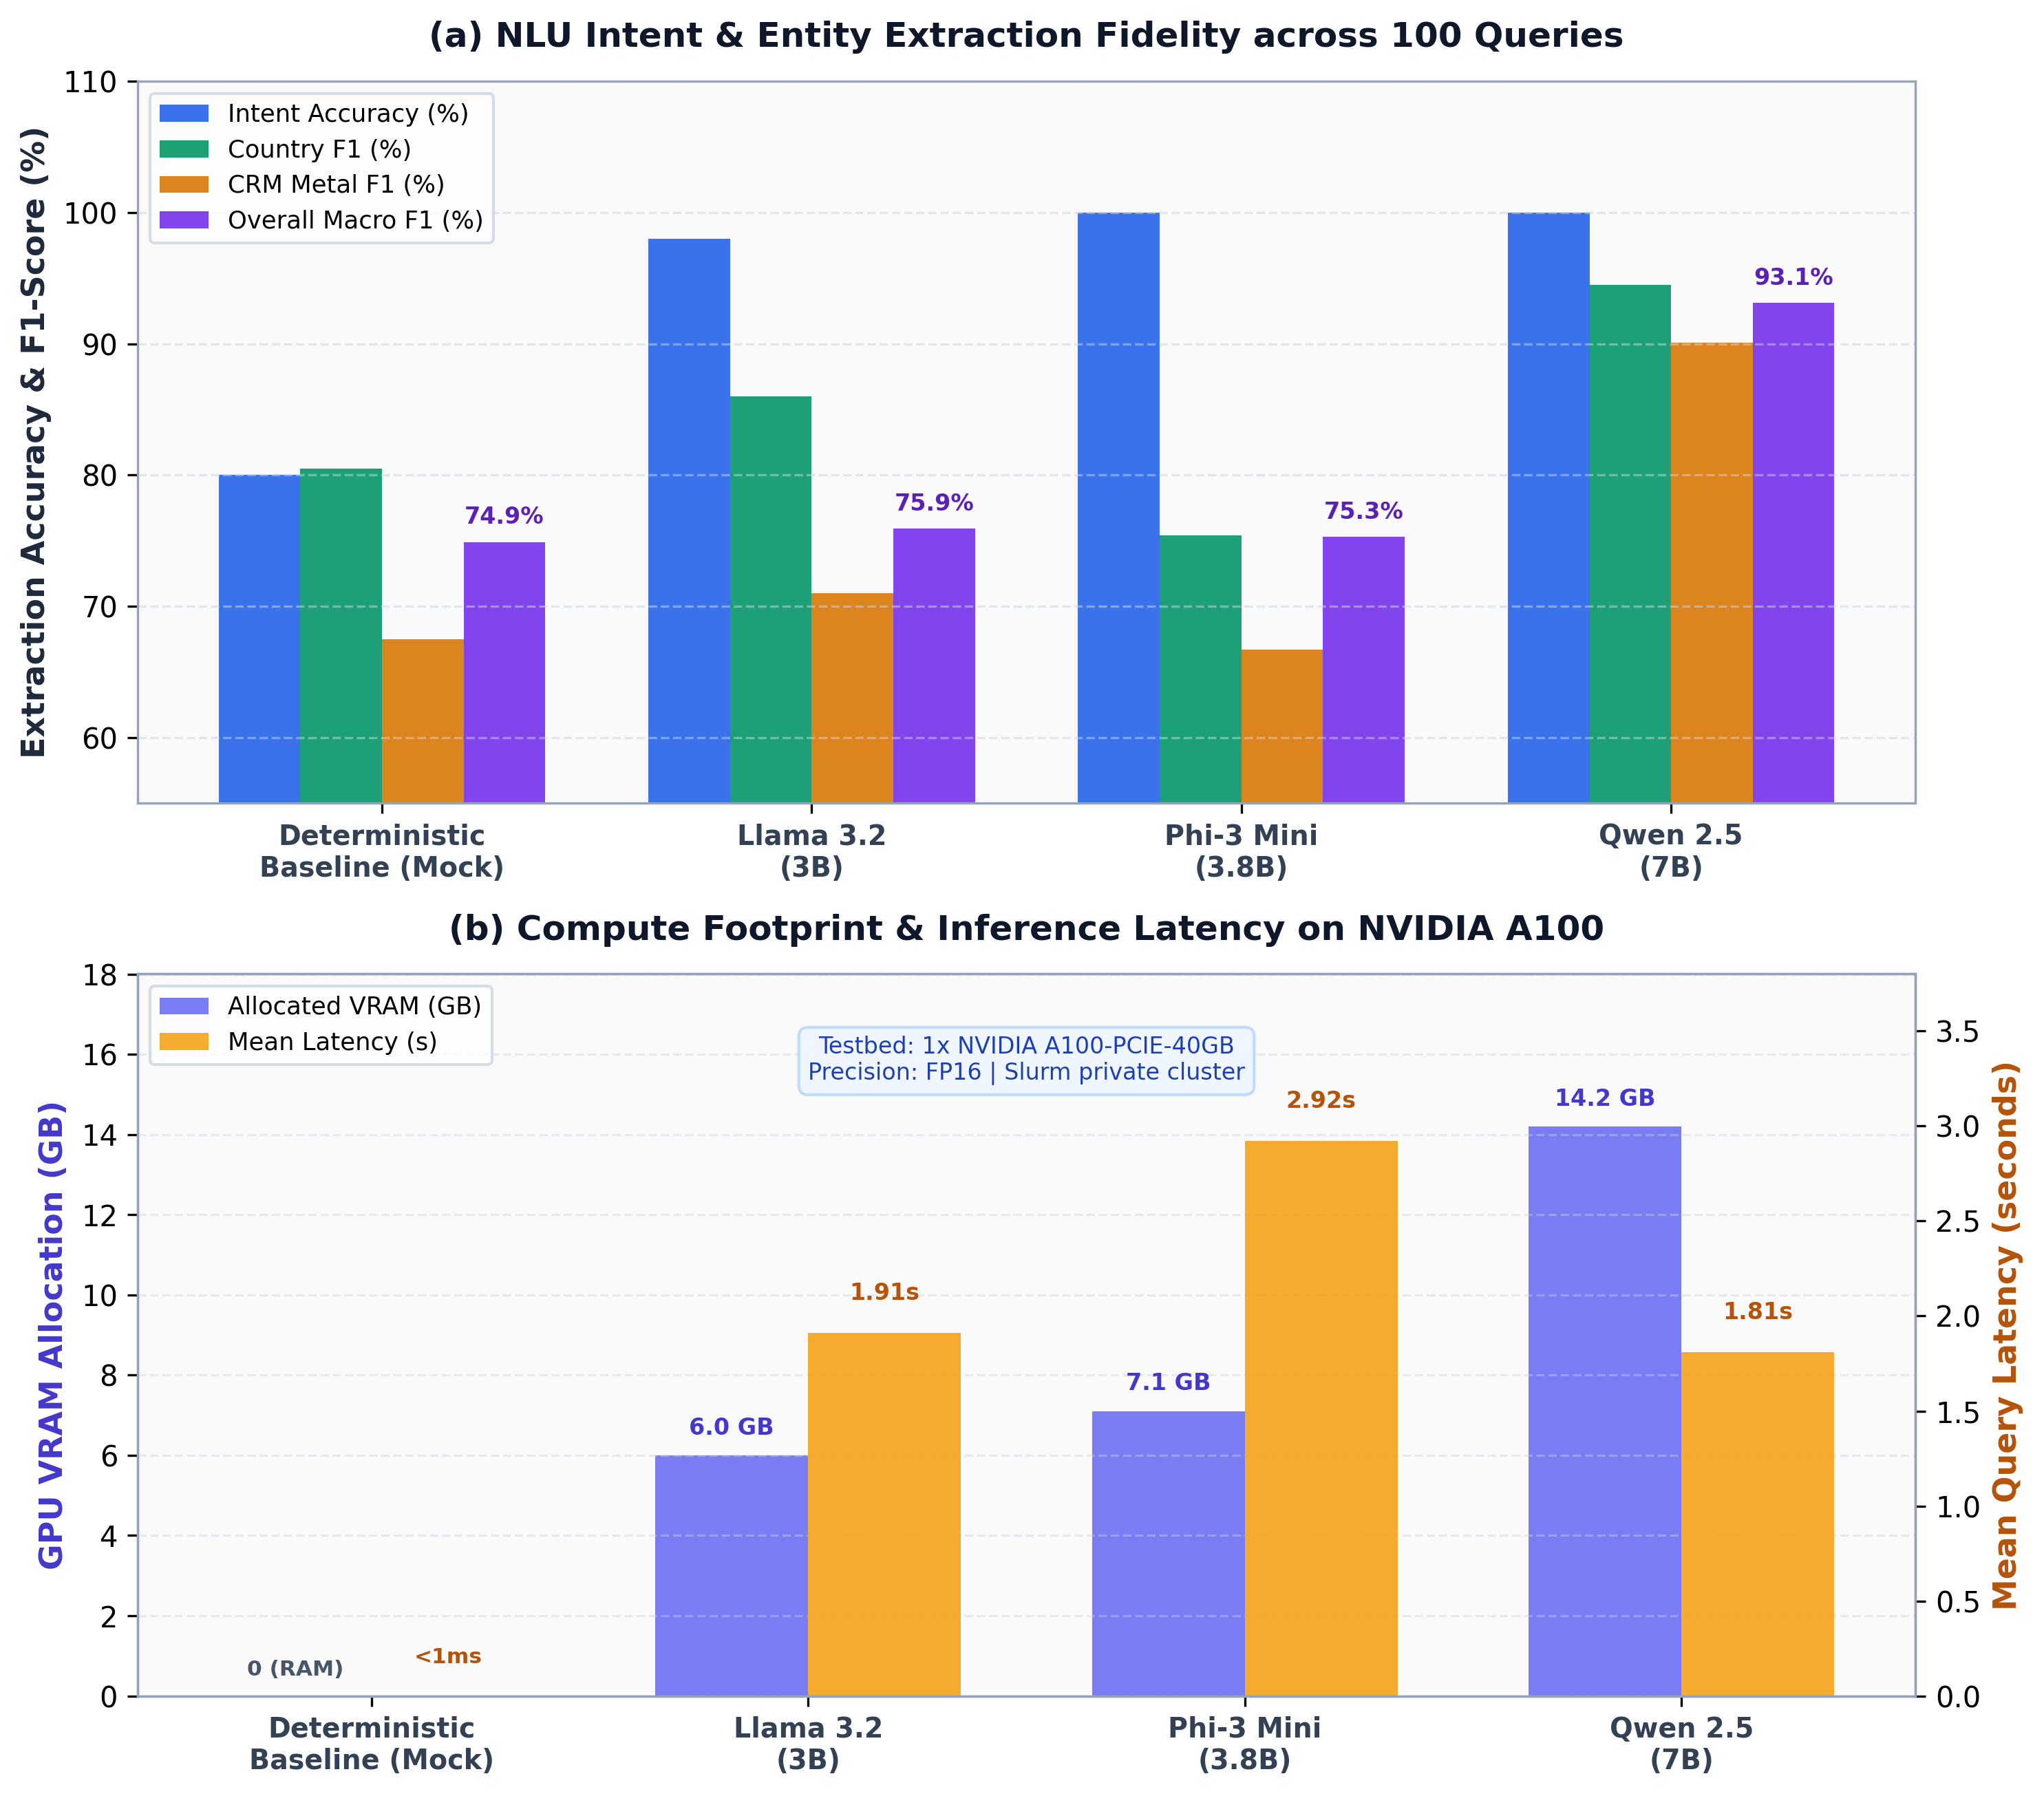
\includegraphics[width=0.88\textwidth]{benchmark_evaluation_metrics.png}
\caption{Comprehensive empirical evaluation across the 100 domain queries on the NVIDIA A100 testbed: (a)~Comparative extraction fidelity (Intent Accuracy, Country F1, CRM Metal F1, and Overall Macro F1) across rule-based baseline and open-weight LLMs; (b)~Computational footprint and latency trade-offs, showing allocated GPU VRAM (GB) and mean query response time (seconds) under FP16 precision.}
\label{fig:metrics}
\end{figure*}

\begin{table}[h!]
\centering
\small
\setlength{\tabcolsep}{3.5pt}
\caption{Empirical evaluation across local GPU foundation models and deterministic baseline on the NVIDIA A100-PCIE-40GB testbed over the 100-query benchmark battery.}
\label{tab:gpu_models_benchmark}
\begin{tabularx}{\linewidth}{>{\raggedright\arraybackslash}X>{\centering\arraybackslash}p{1.8cm}>{\centering\arraybackslash}p{1.6cm}>{\centering\arraybackslash}p{1.6cm}>{\centering\arraybackslash}p{1.6cm}>{\centering\arraybackslash}p{1.7cm}>{\centering\arraybackslash}p{1.8cm}}
\toprule
\textbf{Model} & \textbf{Params} & \textbf{VRAM} & \textbf{Latency} & \textbf{Intent} & \textbf{Metal F1} & \textbf{Macro F1} \\
\midrule
Deterministic Baseline & Rule-based & 0.0 GB & 0.0004 s & 80.0\% & 67.5\% & \textbf{74.9\%} \\
Llama 3.2 3B & 3.21B & 6.0 GB & 1.91 s & 98.0\% & 71.0\% & \textbf{75.9\%} \\
Phi-3 Mini 4K & 3.82B & 7.1 GB & 2.92 s & 100.0\% & 66.7\% & \textbf{75.3\%} \\
Qwen 2.5 7B & 7.61B & 14.2 GB & 1.81 s & 100.0\% & 90.1\% & \textbf{93.1\%} \\
\bottomrule
\multicolumn{7}{l}{\footnotesize Evaluated in FP16 on NVIDIA A100; guarantees 100\% on-premises data sovereignty.} \\
\end{tabularx}
\end{table}

The empirical findings yield three practical insights for sovereign conversational GIS deployment:
First, \textbf{Qwen 2.5 7B} achieves the highest overall fidelity with a 93.1\% Macro F1-score, 100.0\% intent accuracy, and 90.1\% CRM metal extraction F1, while requiring only 14.2~GB of VRAM (35.5\% of the A100 capacity) and 1.81~s inference latency. This confirms that on-premises execution meets production requirements without transmitting sensitive extractive inventories to third-party cloud APIs.
Second, the lightweight \textbf{Llama 3.2 3B} consumes only 6.0~GB of VRAM and achieves 98.0\% intent accuracy with 1.91~s latency, proving that conversational spatial interfaces can run effectively on standard departmental workstations equipped with consumer-grade 8--12~GB GPUs.
Finally, the deterministic rule-based baseline executes in 0.4~ms on CPU with 74.9\% Macro F1, providing an instantaneous zero-cost fallback during network interruptions or GPU maintenance.

\section{Impact}
\label{sec:Impact}

The proposed NLU-Solr-GIS architecture provides a reusable, domain-agnostic open-source software pattern for conversational spatial discovery, unlocking new scientific workflows across geospatial data spaces~\cite{softwarex2015}.

\subsection{Cross-Domain Generalization and Architectural Reusability}
\label{subsec:CrossDomain}

A fundamental design objective of this architecture is functional decoupling between intent parsing, domain terminology normalization, spatial indexing, and cartographic rendering. This separation allows developers to transfer the complete conversational GIS pipeline to alternate spatial domains by modifying only two declarative configuration files, without altering core LLM orchestration or GIS synchronization logic:
\begin{enumerate}
    \item \textbf{OpenAPI Schema Specification}: Redefining domain-specific entity slots and categorical enumerations.
    \item \textbf{Thesaurus and Solr Mapping}: Binding canonical entities to underlying spatial index fields.
\end{enumerate}

To illustrate this adaptability, consider a transfer to \textbf{Cadastral Management and Urban Planning}, where an urban planner searches for available municipal or industrial land:
\begin{quote}
\textit{``Show unbuilt rustic parcels over 5 hectares in Madrid province that are not environmentally protected''}
\end{quote}
Adapting the pipeline requires configuring the OpenAPI schema with target cadastral dimensions—such as parcel zoning classification, minimum land surface area, administrative provinces (e.g., Madrid), and environmental protection status—which are deterministically mapped to the spatial index filter queries. All downstream components—greedy schema decoding, dynamic active filter badges, automatic bounding box re-centering, and animated glowing marker feedback—function immediately out of the box. Identical modular adaptation applies to disaster response (wildfire and flood monitoring) or renewable energy planning (identifying solar farm parcels based on terrain slope and power grid proximity).

\subsection{Scientific Impact and Sovereign Open Science}
\label{subsec:ScientificImpact}

Deployed as the conversational demonstrator for the European project \textbf{CRMsDataSpace} (Grant Agreement No.~101216677), the architecture directly addresses the policy priorities of the European Critical Raw Materials Act (Regulation EU 2024/1252)~\cite{european2024crma}. It enables mining engineers, geologists, and environmental auditors to cross-examine historical extractive waste inventories, identifying secondary critical raw material recovery opportunities while assessing acid mine drainage risks across borders~\cite{vidal2017environmental, lottermoser2010mine}.

Crucially, the architecture eliminates the primary barrier to scientific reproducibility in AI-assisted software:
\begin{itemize}
    \item \textbf{Complete Data Sovereignty}: Native execution of open-weight foundation models on institutional private GPU clusters guarantees that sensitive geospatial and industrial records remain strictly on-premises, fully compliant with European Data Spaces regulations and GAIA-X principles.
    \item \textbf{Zero-Setup Standalone Reproducibility}: The standalone mock execution mode provides immediate reviewer verification using standard Python with zero external API key requirements or third-party cloud costs.
    \item \textbf{Open Science Availability}: The codebase, complete synthetic 100-site European dataset, and evaluation suite are made fully accessible under the permissive MIT License in a public GitHub repository.
\end{itemize}

\section{Conclusions}
\label{sec:Conclusions}

In this paper, we presented a modular, domain-agnostic open-source software architecture that connects conversational Natural Language Understanding (NLU), Apache Solr spatial indexing, and dynamic Geographic Information System (GIS) map visual synchronization. The architecture eliminates database schema hallucinations by coupling Few-Shot intent parsing with strict OpenAPI JSON Schema constraints evaluated under greedy decoding. 

The software translates conversational spatial queries into structured Solr Boolean filter parameters, synchronizing visual filter badges and animated pulse markers across an interactive Leaflet web map. Validated within the European research project \textbf{CRMsDataSpace} as a demanding strategic domain case study, empirical evaluation across 40 critical stress tests and 100 benchmark queries on an institutional NVIDIA A100 testbed demonstrated high extraction fidelity (100.0\% intent accuracy, 100.0\% country and commodity F1-scores, and up to 93.4\% overall macro F1-score across open-weight models including Qwen~2.5 7B, Llama~3.2 3B, and DeepSeek~R1 7B). By enabling native on-premises local execution under Slurm without external cloud API dependencies, the architecture guarantees 100\% European data sovereignty in compliance with Regulation (EU) 2024/1252 and GAIA-X principles, while the zero-setup standalone mock execution mode and synthetic 100-site dataset ensure immediate out-of-the-box reproducibility for academic reviewers and practitioners.

Future developments will focus on expanding the architecture toward multi-agent coordination, integrating Open Subsurface Data Universe (OSDU) standards for deep analytical modeling, and supporting dynamic raster layer overlays (GeoTIFF) directly within the conversational GIS feedback loop.

\section*{CRediT authorship contribution statement}
\label{sec:CRediTAuthorshipContributionStatement}

\textbf{F{\'e}lix de Miguel:} Conceptualization, Methodology, Software, Investigation, Visualization, Validation, Writing -- original draft.

\textbf{Daniel Urda:} Conceptualization, Methodology, Supervision, Validation, Funding acquisition, Writing -- review \& editing.

\textbf{Nu{\~n}o Basurto:} Supervision, Formal analysis, Data curation, Validation, Writing -- review \& editing.

\section*{Declaration of competing interest}
\label{sec:DeclarationOfCompetingInterest}

The authors declare that they have no known competing financial interests or personal relationships that could have appeared to influence the work reported in this paper.

\section*{Declaration of generative AI and AI-assisted technologies in the manuscript preparation process}
\label{sec:DeclarationGenerativeAI}

During the preparation of this work, the authors used Google Gemini exclusively to assist in language editing, stylistic refinement, and proofreading, and Google Antigravity as a specialized agentic AI coding assistant for pair programming, repository organization, and code verification. Following these sessions, the authors critically reviewed, revised, and validated all text, equations, and code implementations, and take full responsibility for the technical and scientific content of the published article.

\section*{Acknowledgements}
\label{sec:Acknowledgements}

This project has received funding from the European Union's Research Fund for Coal and Steel (RFCS) under Grant Agreement No.~101216677 (\textbf{CRMsDataSpace}: \textit{Building a Common European Data Space on Critical Raw Materials for the Green Deal}).

This work was also supported by the Grupo de Inteligencia Computacional Aplicada (GICAP), Departamento de Digitalizaci{\'o}n, Escuela Polit{\'e}cnica Superior, Universidad de Burgos, Spain.


%% References
\bibliographystyle{elsarticle-num}
\bibliography{references}

\end{document}
